% !TeX root = ../../main.tex

\chapter{Stand der Technik}

\section{Was ist Photogrammetrie?}
Mit Photogrammetrie bezeichnet man Techniken, mit denen man Informationen wie Position, Orientierung, Form und Größe eines Objekts aus Bildern rekonstruieren kann.
Dabei unterscheidet man ob es sich bei den Bildern um photochemische (konventionelle Photographie), photoelektrische (digitale Photographie) oder um Laserscanner-Aufnahmen, dabei handelt es sich um Bilder welche zusätzlich Entfernungsinformationen zu jedem Bildelement enthalten, handelt.
Je nach Art der Weiterverarbeitung sowie Aufnahme der Bilder wird der Begriff der Photogrammetrie weiter differenziert.
Bei Weiterverarbeitung von photochemischen Bildern mittels optisch-mechanischer Geräte spricht man von \textbf{analoger Photogrammetrie}.
Bei Weiterverarbeitung von photochemischen Bildern mittels Computer spricht man von \textbf{analytischer Photogrammetrie}.
Bei Weiterverarbeitung von photoelektrischen Bildern mittels Computer, ein voll digitaler Prozess, spricht man von \textbf{digitaler Photogrammetrie}.
Die Ergebnisse einer Auswertung mittels Photogrammetrie können sein: \cite{kraus_2004}
\begin{itemize}
\item \textbf{Maßzahlen}, Koordinaten einzelner Objektpunkte in einem dreidimensionalen Koordinatensystem
\item \textbf{Zeichnungen}, Karten und Pläne im Grundriss mit Höhenlinien
\item \textbf{geometrische Modelle}
\item \textbf{Bilder}, entzerrte Fotos, Luftbildkarten
\end{itemize}

In dieser Arbeit werden Techniken der digitalen Photogrammetrie verwendet mit dem Ziel Maßzahlen als Ergebnis zu erhalten.
 


\section{Definitionen \& Begriffe}
\subsection{Structure from Motion}\label{sec:sfm}
Unter Structure from Motion, kurz SfM, 
zitat opencv dokument zu SfM

\subsection{Lochkamera-Modell}\label{sec:pinhole-camera-model}
Das Lochkamera-Modell ist das einfachste Kameramodell und wird im Folgenden dazu verwendet relevante Begriffe und die Geometrie zu erklären.
Bei diesem Modell wir die zentrale Projektion von Punkten im Raum auf eine Ebene betrachtet.
Das Zentrum der Projektion definiert den Ursprungs eines euklidischen Koordinatensystems.
Der Ursprung wird auch \emph{Kamerazentrum} genannt und als Punkt $C$ referenziert.
Die Bildebene liegt parallel zu der XY-Ebene auf der Z-Achse.
Der Abstand zum Ursprung wird durch die Brennweite $f$ der Kamera definiert.
Der Schnittpunkt $p$ der Bildebene und der Z-Achse wird als Hauptpunkt (engl. principal point) bezeichnet.
Der Hauptpunkt definiert innerhalb der Bildebene den Ursprung eines zweidimensionalen Koordinatensystems.
Häufig ist es aber der Fall, dass der Hauptpunkt und der Ursprung voneinander abweichen.
Daher wird der Ursprung auch mit den Koordinaten $(p_x, p_y)^T$ angegeben.
Mit diesen Informationen kann nach~\cite[Gleichung 6.2]{hartley_2003} die Abbildung eines Punkts im Raum auf die Bildebene in homogenen Koordinaten durch eine Matrixmultiplikation ausgedrückt werden:
\begin{equation}
\label{eqn:theory-projection}
\begin{pmatrix}
    X \\ Y \\ Z \\ 1
\end{pmatrix}
\mapsto
\begin{pmatrix}
    fX+Zp_x \\ fY+Zp_y \\ Z
\end{pmatrix}
=
\begin{bmatrix}
    f &   & p_x & 0 \\
      & f & p_y & 0 \\
      &   & 1   & 0
\end{bmatrix}
\begin{pmatrix}
    X \\ Y \\ Z \\ 1
\end{pmatrix}
\end{equation}
Diese Gleichung lässt sich mit der Notation $X$ für einen homogenen 4-Vektor, $x$ für einen homogenen 3 Vektor als $x = PX$ schreiben.
Dabei ist $P$ die homogene $3\times 4$ \emph{Kamera-Projektionsmatrix} (auch \emph{Kamermatrix} oder \emph{Projektionsmatrix} genannt).
Mit der Definition der \emph{Kamera-Kalibrierungsmatrix} (auch \emph{Kalibrierungsmatrix}) K
\[
    K=
    \begin{bmatrix}
    f &   & p_x & 0 \\
      & f & p_y & 0 \\
      &   & 1   & 0
    \end{bmatrix}
\]
kann die~\ref{eqn:theory-projection} auch zu $x=K[I | 0] X$ vereinfacht werden~\cite[vgl. Gleichung 6.5]{hartley_2003}. 


\begin{figure}
    \centering
    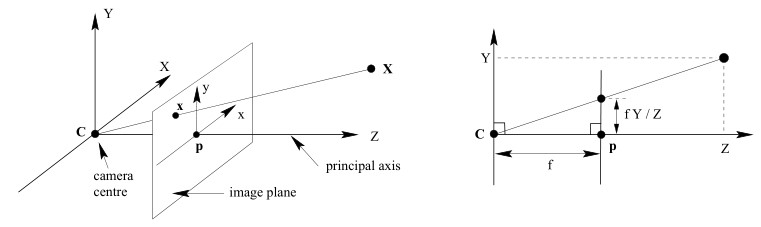
\includegraphics[width=\textwidth]{src/img/hartley_2003_lochkamera.jpg}
    \caption{Darstellung des Lochkamera-Modells~\cite[Fig. 6.1]{hartley_2003}}
    \label{fig:theory-pinhole-camera}
\end{figure}


Für gewöhnlich werden Punkte in einem Raum in einem anderem Koordinatensystem ausgedrückt.
Die Beziehung zwischen beiden Koordinatensystemen wird durch die $3\times 3$ Rotationsmatrix $R$ und dem Translationsvektor $t$ beschrieben. 
Die Kamera-Projektionsmatrix kann somit auch als $P=K[R|t]$ geschrieben werden~\cite[Kapitel 6.1,S. 156, Gleichung 6.7]{hartley_2003}.


\subsection{Fundamental Matrix}
Die Fundamental Matrix ist eine algebraische Darstellung der Epipolargeometrie zwischen zwei Sichten.
Ziel dieser Geometrie ist die Suche von korrespondierenden Punkten in zwei Sichten.

Man nehme an, dass der Raumpunkt $X$, die Bildpunkte $x$ und $x'$, und die Kamerazentren $C$ und $C'$ in einer Ebene, genannt $\pi$, liegen (siehe Abb.~\ref{fig:theory-fundamental-matrix}).
Man erkennt, dass sich die Linien von den Kamerazentren durch $x$ bzw. $x'$ in $X$ schneiden und ebenfalls in der Ebene liegen.
Mit dieser Eigenschaft kann man die Suche von korrespondierenden Bildpunkten vereinfachen.
Nimmt man an, dass man nur den Bildpunkt $x$ kennt, dann kann man mit Hilfe der Ebene $\pi$ die Position von $x'$ einschränken.
Denn $x'$ muss sich auf der Schnittlinie der eben beschriebenen Ebene und der Bildebene der zweiten Sicht befinden. 
Diese Schnittlinie wird \emph{Epipolarlinie} genannt.
Die Punkte $e$ und $e'$ sind die Schnittpunkte des Vektors $\overline{CC'}$ mit den Bildebenen und werden Epipole genannt.
Die Ebene $\pi$ wird zusätzlich Epipolarebene genannt~\cite[Kapitel 9,1]{hartley_2003}.

% S.240 / 241 multiple view geometry
Die Fundamental Matrix wird in~\cite[Kapitel 9.2]{hartley_2003} definiert als die $3\times 3$ Matrix, die für alle korrespondierenden Punkte $x \leftrightarrow x'$ 
\[ x'^TFx=0\] 
erfüllen.
Geometrisch betrachtet ist die Matrix F eine Abbildung der Punkte in einem Bild auf ihre Epipolarlinien im zweiten Bild.

\begin{figure}[h!]
    \centering
    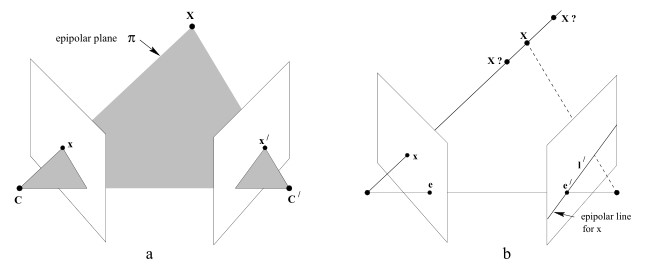
\includegraphics[width=\textwidth]{src/img/hartley_2003_fundamental_matrix.jpg}
    \caption{Veranschaulichung der Epipolargeometrie~\cite[Fig. 9.1]{hartley_2003}}
    \label{fig:theory-fundamental-matrix}
\end{figure}

\subsection{Essentielle Matrix}
Die essentielle Matrix ist eine Spezialisierung der Fundamentalmatrix mit normalisierten Bildkoordinaten.
Sie wird durch die Gleichung $\hat{x}'E\hat{x}$ definiert, wobei $\hat{x}$ ein Punkt in normalisierten Bildkoordinaten darstellt.
Mit Hilfe der Kalibrierungsmatrizen $K$ und $K'$ von zwei Bildern, kann die Beziehung $E=K'^TFK$ zur Fundamentalmatrix hergeleitet werden~\cite[Kapitel 9.6]{hartley_2003}.

Es ist möglich durch eine Singulärwertzerlegung der essentiellen Matrix die Kameramatrix zu bestimmen.
Dabei wird für die erste Kameramatrix $P=[I|0]$ angenommen. 
Für die zweite Kameramatrix gibt es vier Möglichkeiten, die sich aus den zwei möglichen Rotationsmatrizen $R$ und den zwei möglichen Vorzeichen für den Translationsvektor $t$ ergeben.
Geometrisch betrachtet kann jedoch nur einer der Kombinationen stimmen.
Wie in Abb.~\ref{fig:theory-essential-matrix-geometry} zusehen ist, gibt es nur einen Fall, bei dem ein Punkt im Raum vor beiden Bildebenen liegt.
Mit dieser Überprüfung kann die zweite Kameramatrix $P'=[R|t]$ bestimmt werden.
Hier muss beachtet werden, dass $t$ ein Einheitsvektor und nur maßstabsgetreu ist~\cite[Kapitel 9.6.3]{hartley_2003}.


\begin{figure}[h!]
    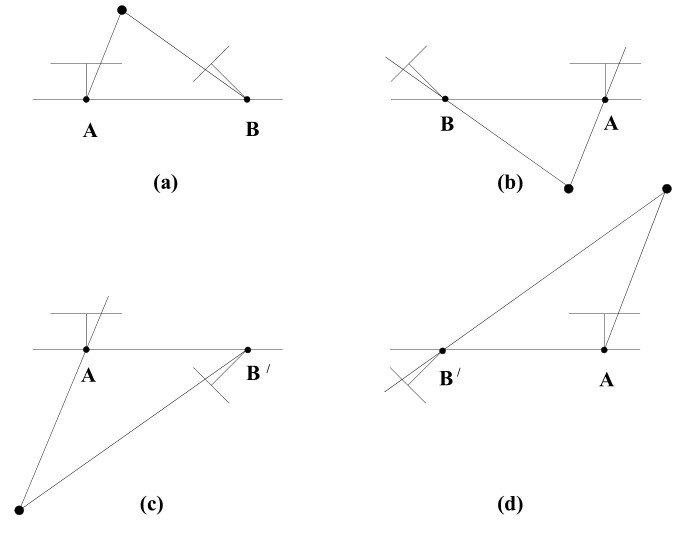
\includegraphics[width=\textwidth]{src/img/hartley_2003_e_geometry.jpg}
    \caption{Die geometrische Darstellung der vier möglichen Lösungen für $E$. Nur in (a) liegt der markierte Punkt vor beiden Kameraebenen~\cite[Fig. 9.12]{hartley_2003}}.
    \label{fig:theory-essential-matrix-geometry}
\end{figure}

\section{Kamerakalibrierung}
Die Kamerakalibrierung ist ein Prozess zum Bestimmen der kamera-spezifischen Parametern der Kameramatrix und den Verzerrungsparametern. 
Die Kameramatrix wird in \cref{sec:pinhole-camera-model} erklärt.
Die Verzerrungsparameter werden genutzt, um die Verzerrung auszugleichen, die durch der Kameralinse entsteht.
Hierbei wird zwischen zwei Arten der Verzerrung unterschieden: radiale und tangentiale Verzerrung.
Radiale Verzerrung entsteht durch die runde Form der Linse, wodurch die Pixel am Bildrand verzerrt werden.
Diese Verzerrung kann bei manchen Linsen zunehmen, je weiter ein Strahl entfernt vom Zentrum auf die Linse trifft. 
Diese Art der Verzerrung kann mathematisch als Taylorreihe um $r = 0$ und dem Termen $k_1, k_2$ und $k_3$ beschrieben werden.
Ein Punkt $(x, y)$ kann somit als $(x_{\text{corrected}},y_{\text{corrected}})$ ohne Verzerrung ausgedrückt werden, wobei gilt:
\[x_\text{corrected} = x \cdot (1 + k_1r^2 + k_2r^4 + k_3r^6)\]
\[y_\text{corrected} = y \cdot (1 + k_1r^2 + k_2r^4 + k_3r^6)\]
Tangentiale Verzerrung entsteht durch Herstellungsfehler, wodurch die Linse nicht genau parallel zur Abbildungsebene liegt.  
Sie wird durch die Parameter $p_1$ und $p_2$ beschrieben, wodurch ein Punkt $(x,y)$ durch $(x_{\text{corrected}},y_{\text{corrected}})$ ohne Verzerrung dargestellt wird. 
Dabei gilt:
\[x_\text{corrected} = x + (2p_1xy + p_2(r^2 + 2x^2))\]
\[y_\text{corrected} = y + (p_1(r^2 + 2y^2) + 2p_xy)\]
\cite{kaehler_2016}

Eine Kamera kann mit verschieden Methoden kalibriert werden.
Häufig werden bei den Methoden Referenzraster eingesetzt, wie z.B.\ ein Schachbrettmuster.
Das Referenzraster kann hierbei 2D oder auch 3D sein wie in den \cref{fig:2d_grid,fig:3d_grid} zu sehen ist.
Eine weitere Methode ist die Auto-Kalibrierung, bei der kein Kalibrierungsobjekt genutzt wird.
Dabei werden die Kameraeigenschaften aus unkalibrierten Bildern gewonnen, in dem Restriktionen auf die Kameraparameter oder auf die abgebildete Szene gelegt werden.
Die Auto-Kalibrierung wird häufig bei der 3D Modellierung eingesetzt~\cite{remondino_2005}.

\begin{figure}[h]
    \centering
    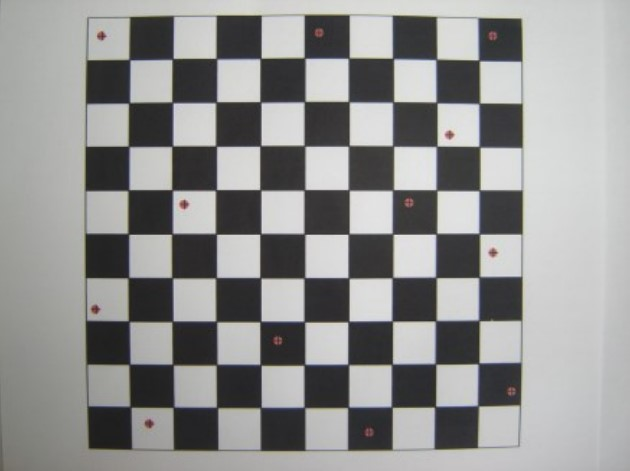
\includegraphics[width=\textwidth]{src/img/mendonca_2013_2d_grid.jpg}
    \caption{2D Referenzraster mit Schachbrettmuster für die Kamerakalibrierung (aus~\cite[Fig. 2]{mendonca_2013})}
    \label{fig:2d_grid}
\end{figure}



\begin{figure}[h]
    \centering
    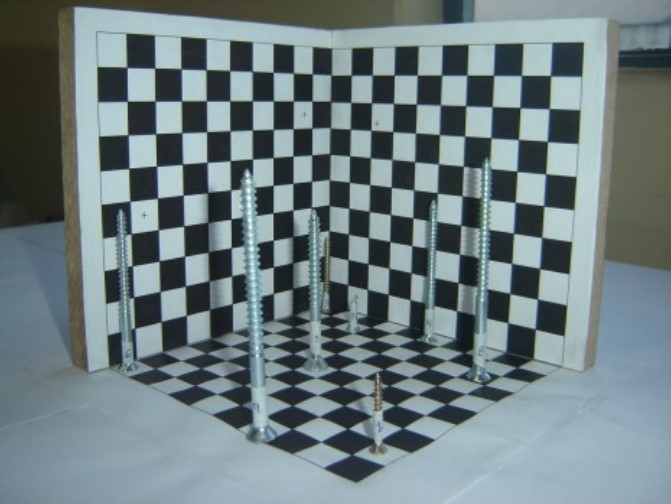
\includegraphics[width=\textwidth]{src/img/mendonca_2013_3d_grid.jpg}
    \caption{3D Referenzraster mit Schachbrettmuster für die Kamerakalibrierung (aus~\cite[Fig. 4]{mendonca_2013})}
    \label{fig:3d_grid}
\end{figure}

